\documentclass{ubicomp-ext}
\usepackage{libertine} % for the pretty dark-circle-enclosed numbers
\usepackage{tikz}
\usepackage{float}
\usepackage{listings}
\usepackage{multicol}
\usepackage{color}
\usepackage{minibox}
\usepackage{fancybox}
\usepackage{fontspec}
\usepackage{ifthen}
\newfontfamily{\lstsansserif}[Scale=.7]{Arial}
\newfontfamily{\textlst}{Arial}
\definecolor{Lemon}{HTML}{FFFACD}
\newcounter{lstNoteCounter}
\newcommand{\lnnum}[1]
    {\ifthenelse{#1 =  1}{\libertineGlyph{uni2776}}
    {\ifthenelse{#1 =  2}{\libertineGlyph{uni2777}}
    {\ifthenelse{#1 =  3}{\libertineGlyph{uni2778}}
    {\ifthenelse{#1 =  4}{\libertineGlyph{uni2779}}
    {\ifthenelse{#1 =  5}{\libertineGlyph{uni277A}}
    {\ifthenelse{#1 =  6}{\libertineGlyph{uni277B}}
    {\ifthenelse{#1 =  7}{\libertineGlyph{uni277C}}
    {\ifthenelse{#1 =  8}{\libertineGlyph{uni277D}}
    {\ifthenelse{#1 =  9}{\libertineGlyph{uni277E}}
    {\ifthenelse{#1 = 10}{\libertineGlyph{uni277F}}
    {\ifthenelse{#1 = 11}{\libertineGlyph{uni24EB}}
    {\ifthenelse{#1 = 12}{\libertineGlyph{uni24EC}}
    {\ifthenelse{#1 = 13}{\libertineGlyph{uni24ED}}
    {\ifthenelse{#1 = 14}{\libertineGlyph{uni24EE}}
    {\ifthenelse{#1 = 15}{\libertineGlyph{uni24EF}}
    {\ifthenelse{#1 = 16}{\libertineGlyph{uni24F0}}
    {\ifthenelse{#1 = 17}{\libertineGlyph{uni24F1}}
    {\ifthenelse{#1 = 18}{\libertineGlyph{uni24F2}}
    {\ifthenelse{#1 = 19}{\libertineGlyph{uni24F3}}
    {\ifthenelse{#1 = 20}{\libertineGlyph{uni24F4}}
    {NUM TOO HIGH}}}}}}}}}}}}}}}}}}}}}


\newcommand{\lstref}[1]{\lnnum{\ref{#1}}}

\newcommand{\lstnote}[1] {
\label{#1}\vbox{\llap{{\lnnum{\ref{#1}}}\hskip 1em}}
}

\lstnewenvironment{csource}[1][]
{
 \setcounter{lstNoteCounter}{0}
 \lstset{basicstyle=\lstsansserif, frame=lines, framexleftmargin=0.5em,
            framexrightmargin=0.5em, backgroundcolor=\color{Lemon}, showstringspaces=false, escapeinside={(*@}{@*)}, #1}
}{}
% Please be sure that you have the dependencies (i.e., additional LaTeX packages) to compile this example.

\copyrightinfo{
  Copyright is held by the author/owner(s).\\
  {\emph{UbiComp '13 Adjunct}}, Sept 8-12, 2013, Zurich, Switzerland.\\
  ACM 978-1-4503-2139-6/13/09...\$15.00.
}

\title{Torwads Context-Oriented Programming in Wireless Sensor Networks}

\numberofauthors{8}
% Notice how author names are alternately typesetted to appear ordered in 2-column format;
% i.e., the first 4 autors on the first column and the other 4 auhors on the second column.
% Actually, it's up to you to strictly adhere to this author notation.
\author{
  \vspace{-1.5em} % lisatolles: The abstract heading should start at the time height on the page as the authors names
  \alignauthor{
  	\textbf{First Author}\\
  	\affaddr{AuthorCo, Inc.}\\
  	\affaddr{123 Author Ave.}\\
  	\affaddr{Authortown, PA 54321 USA}\\
  	\email{author1@anotherco.com}
  }\alignauthor{
  	\textbf{Fifth Author}\\
  	\affaddr{AuthorCo, Inc.}\\
  	\affaddr{123 Author Ave.}\\
  	\affaddr{Authortown, PA 54321 USA}\\
  	\email{author5@anotherco.com}
  }
  \vfil
}

% Paper metadata (use plain text, for PDF inclusion and later re-using, if desired)
\def\plaintitle{UbiComp 2013 LaTeX Extended Abstracts Template}
\def\plainauthor{Luis A. Leiva}
\def\plainkeywords{Guides, instructions, author's kit, conference publications}
\def\plaingeneralterms{Documentation, Standardization}

\hypersetup{
  % Your metadata go here
  pdftitle={\plaintitle},
  pdfauthor={\plainauthor},  
  pdfkeywords={\plainkeywords},
  pdfsubject={\plaingeneralterms},
  % Quick access to color overriding:
  %citecolor=black,
  %linkcolor=black,
  %menucolor=black,
  %urlcolor=black,
}

\usepackage{graphicx}   % for EPS use the graphics package instead
\usepackage{balance}    % useful for balancing the last columns
\usepackage{bibspacing} % save vertical space in references


\begin{document}

\maketitle

\begin{abstract}
  We present our ongoing work towards applying the context-oriented
  programming paradigm to wireless sensor networks
  (WSNs). Context---as a representation of the environment where the
  system operates---plays a key role in WSNs. For example, WSN
  applications must often adapt their operation depending on
  environmental data. We argue that promoting a notion of context as a
  first-class citizen in WSN programming facilitates the design and
  implementation of context-dependent functionality. To this end, we
  conceive a context-oriented programming model expressly tailored to
  WSNs, coupled with dedicated language constructs. Unlike the
  existing literature on context-oriented programming, we embed the
  latter within low-level C-like languages that do not rely on
  resource-intensive features such as dynamic memory management. To
  make our design concrete, we describe a context-oriented extension
  of nesC, a widely used WSN programming language, and report on a
  preliminary assessment of our design.

% Programming for embedded systems makes a significant part in the modern software development. Despite the rapid growth of the high-level languages there are still a necessity to use embedded systems. The prime example of this are Wireless Sensor Networks (WSNs). Most of the platforms for them are embedded.

% The main task of WSNs is to monitor the environment. Thus, they are widely applied in different areas, such as health monitoring, wildlife tracking, smart home etc. But the environment is changing very fast, so it is necessary to react to these changes. In order to make WSN to be aware of changes we have to use a representation of the state of the environment within the WSN. In other words, we have to use \textit{Context} in programming for WSNs.

% \textit{Context} could be defined as an entity, which represents a state of the environment. It can be used as a simplified model of the environment and could be formed according to sensing data. It is possible to develop more autonomous and more flexible system by using \textit{Contexts} in programming for WSNs.

% Context-oriented programming (COP) is a programming technique which makes it possible to create an adaptive software by using \textit{Context} as an information about the state. Such a software could adapt to changes in the environment and to evolve according to this changes. The term ``evolve'' means that software can change behaviour and this behaviour depends on the context in which it is executed.

% In this work we show how COP could be used for programming for embedded platforms and for WSNs in particular. We overview an example of the possible application of the WSN, then we extract the structure of the context for this application to highlight the specific aspects of the context-oriented approach in embedded systems. In the end we propose a small extension of the existing language for WSNs.
\end{abstract}
% =============================================================================
\section{Introduction}
% =============================================================================
Wireless Sensor Networks (WSNs) can be applied in different areas \cite{pastor08}. In this paper we use Smart Home as a particular example. This application of WSN have to track householder location and execute a list of instructions depending on it. In parallel, WSN should monitor and control a climate in the house. On the hardware level WSN have sensors to monitor the environment (like temperature, light intensity etc.), which are static. There are also mobile sensors, which are attached to the householder to track his location inside and outside the house. In order to ensure an appropriate quality of service, they should provide a long work time and be as autonomous as possible. These requirements lead to very complex source code. To reduce the complexity we propose to use Context-Oriented paradigm.

\marginpar{
  \begin{figure}
    \centering
    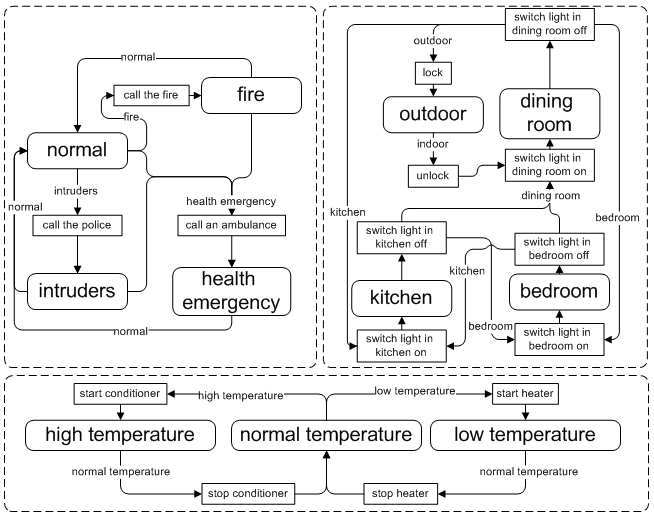
\includegraphics[width=\marginparwidth]{smarthome.png}
    \caption{Context diagram for Smart Home WSN.}
    \label{fig:cdsm}
  \end{figure}
}

Context can be defined as ``any information that can be used to characterize the situation of an entity, where an entity can be a person, place or physical object" \cite{dey99}. Context-Oriented Programming (COP) \cite{hirschfeld08} is an approach which provides an opportunity for a programmer to develop a software which can dynamically change the behaviour depending on the activated context.Using \textit{context} as a building block programmer could easily create an application for WSN, which is aware of changes in the environment.

Thus, COP could be used as an effective way to use a \textit{Context} for developing a software for WSNs. It also will help to avoid the increasing complexity of a program. In our example (Smart Home) there are a lot of possible \textit{contexts}, which are depending on the type of sensor, state of the environment and location of the householder. Some of \textit{contexts} are mutually exclusive, while other can be activated in parallel. For example, usually householder can not move from bathroom directly outside the house, thus this kind of the location change should be treated as an error. But climate state does not depend on the householder's location and corresponding \textit{contexts} can be activated or deactivated independently.

Considering a description of possible context in Smart Home, bringing COP into WSNs is accompanied by following challenges.
\begin{itemize}\compresslist
\item
In WSNs \textit{contexts} could have complex interactions and interconnections. It is necessary to use a specific for WSNs context-oriented technique.
\item
Languages for embedded platforms are mostly static, there are no tools for object-oriented or dynamic programming. Therefore, COP approaches for high-level languages (like Java, C++ or Python) are not applicable.
\item
Embedded platforms also have restrictions on a hardware level, such as low memory, power consumption constraints, low CPU performance.
\end{itemize}

In this work we are proposing a COP technique for WSNs, which meets the challenges described above. Based on the concepts of the technique, which are described below, we developed a language called {\textlst{ConesC}} as a context-oriented extension of nesC language.
% =============================================================================
\section{ConesC}
% =============================================================================
In {\textlst{ConesC}} we divided contexts into groups. It brings COP on a new level of abstraction and makes it possible to operate complex structures of contexts as a superposition of smaller substructures. Thus, every WSNs could have several mostly independent groups of contexts. Context transitions within the group are initiated by triggers and can be performed only if particular conditions are satisfied. There are also actions which should be performed before activation and after deactivation of the context.

Figure \ref{fig:cdsm} utilises our concepts of {\textlst{ConesC}} and represents a structure of contexts for Smart Home. In this application two context groups could be found: \textit{Location} group and \textit{Temperature} group.

\paragraph{Householder's location.} While householder is moving from one room to another, the system is tracking his location and switching off or on the light in rooms. If householder leaves the house, then \textit{Smart Home} locks the door and unlocks it when householder is nearby.

\begin{Sbox}
\begin{minipage}{\marginparwidth}
\begin{csource}
(*@\textbf{context configuration}@*) Temperature {
(*@\lstnote{layereddef}\textbf{layered}@*) void toggle_leds();}
implementation {
(*@\lstnote{contexts}\textbf{contexts}@*) High, Low,
(*@\lstnote{isdefault}@*) Normal (*@\textbf{is default}@*);
 components LedsC;
 High.Leds -> LedsC;
...
 Error.Leds -> LedsC;}
\end{csource}
\end{minipage}
\end{Sbox}

\marginpar{
  \begin{figure}
    \TheSbox
    \caption{Context configuration component.}
    \label{fig:ccc}
  \end{figure}
}

\begin{Sbox}
\begin{minipage}{\marginparwidth}
\begin{csource}
(*@\textbf{context}@*) High {
(*@\lstnote{transitions}\textbf{transitions}@*) Normal;
 uses interface Leds;}
implementation {
(*@\lstnote{activated}@*)event void activated(){}
(*@\lstnote{deactivated}@*)event void deactivated(){}
(*@\lstnote{check}@*)bool check(){return TRUE;}
(*@\lstnote{layeredimp}\textbf{layered}@*) void toggle_leds(){
  call Leds.set(1);}}
\end{csource}
\end{minipage}
\end{Sbox}

\marginpar{
  \begin{figure}
    \TheSbox
    \caption{Context component.}
    \label{fig:cc}
  \end{figure}
}

\begin{Sbox}
\begin{minipage}{\marginparwidth}
\begin{csource}
(*@\textbf{activate}@*)Temperature.High;
Temperature.toggle_leds();
\end{csource}
\end{minipage}
\end{Sbox}

\marginpar{
  \begin{figure}
    \TheSbox
    \caption{Usage example.}
    \label{fig:ue}
  \end{figure}
}

\paragraph{Climate control.} If the temperature in the room is lower (or higher) than normal, system can enable air heating (or conditioning) to return the temperature to the normal state.

In order to use context-oriented paradigm in nesC, we added new key-words. We are also extended components by \textit{context} and \textit{context configuration}. \textit{Context} is an analogue of \textit{module} and \textit{context configuration} is an analogue of \textit{configuration}. These two components can be used as other components in native nesC-way.

\textbf{Context configuration} component represents a context group (figure \ref{fig:ccc}). It is used to declare layered functions and context included in the group. The behaviour of the layered function (line \lstref{layereddef}) depends on activated context within the current group. Declared functions should be implemented in each declared context. Contexts, which are belonging to the group, are declared by using key-word {\textlst{contexts}} (line \lstref{contexts}). In {\textlst{context configuration}} it is mandatory to declare default context by using a key-word {\textlst{is default}}. This context will be activated just after initialization. In {\textlst{ConesC}} each group of contexts has an {\textlst{Error}} context, which is activated if particular errors have been occurred. This context is generated by the system, but can be overridden by programmer like a {\textlst{context}} component.

\textbf{Context} component (figure \ref{fig:cc}) represents particular context. It is used to define possible transitions, actions before activation and after deactivation, layered functions, and to check transition conditions. To define restrictions for particular context transitions we use key-word {\textlst{transitions}} on the line \lstref{transitions}. In our example it means that only {\textlst{Normal}} can be activated as the next context after {\textlst{High}}. The definition is not mandatory, but if illegal transition will be called, then {\textlst{Error}} context will be activated. If transitions are not defined, any transitions are legal. In {\textlst{ConesC}} it is also possible to define a list of instructions, which should be performed during context transition. It is possible by implementing events {\textlst{activated}} and {\textlst{deactivated}}. Event {\textlst{activated}} (line \lstref{activated}) is fired just before context activation, while event {\textlst{deactivated}} (line \lstref{deactivated}) is fired just after deactivation. However, the implementation of these events is not mandatory. In case of particular conditions of activation for current context, method {\textlst{check}} (line \lstref{check}) should be implemented. If {\textlst{check}} returns {\textlst{FALSE}}, the activation will be ignored and system will remain in the previous state. If method is not defined, conditions will not be verified. On the line \lstref{layeredimp} there is an implementation of the layered function. The implementation is mandatory if the function is declared in the {\textlst{context configuration}}. By calling layered function system choose a specific implementation of that function for the activated context.

The context transition could be triggered by the key-word {\textlst{activate}}. In our example (figure \ref{fig:ue}) this key-word triggers the context transition from the current activated context to the context {\textlst{High}}. Then by calling function {\textlst{Temperature.toggle\_leds()}} system will call the function which was implemented within the context {\textlst{High}}.

{\textlst{Context}} and {\textlst{context configuration}} have nesC-like structure and utilize the same logic. Both components can be used in native nesC way as a regular components.

For a preliminary evaluation we also implemented two simple applications with the same functionality: by using {\textlst{ConesC}} and by using {\textlst{nesC}}. The binary of a program written using {\textlst{ConesC}} is only 2\% bigger than the binary of the program written using {\textlst{nesC}}: 7758 bytes vs 7640 bytes.

\balance
\bibliographystyle{acm-sigchi}
\bibliography{ubicomp}

\end{document}
